\documentclass[11pt,a4paper]{article}

% --- Essential Packages ---
\usepackage[utf8]{inputenc}
\usepackage[margin=0.75in,top=0.75in,bottom=0.75in]{geometry}
\usepackage{graphicx}
\usepackage{xcolor}
\usepackage{listings}
\usepackage{fancyhdr}
\usepackage{titlesec}
\usepackage{booktabs}
\usepackage{enumitem}
\usepackage{float}
\usepackage{hyperref}
\usepackage{microtype}
\usepackage{caption}

% --- Hyperref Setup ---
\hypersetup{
    colorlinks=true,
    linkcolor=black,
    filecolor=black,
    urlcolor=blue,
    pdftitle={Lab Exercise 3 - Implementation of Bingo Game using JavaScript},
    pdfauthor={Danush K (3122247001013)}
}

% --- Color Definitions ---
\definecolor{codebg}{RGB}{248, 249, 252}
\definecolor{tagblue}{RGB}{0, 51, 153}
\definecolor{stringpurple}{RGB}{128, 0, 128}
\definecolor{commentgreen}{RGB}{34, 139, 34}
\definecolor{bordergray}{RGB}{205, 210, 220}

% --- Code Listing Setup for HTML, CSS, and JavaScript ---
\lstdefinelanguage{HTML5}{
    language=html,
    sensitive=true,
    alsoletter={<>=-},
    morecomment=[s]{<!--}{-->},
    morestring=[b]",
    morestring=[b]',
    keywords={DOCTYPE, html, head, title, meta, link, style, body, header, nav, ul, li, a, section, h1, h2, h3, p, b, table, thead, tbody, tr, th, td, form, label, input, select, option, textarea, br, footer, img, div, button, script}
}

\lstdefinelanguage{CSS3}{
    sensitive=false,
    morecomment=[s]{/*}{*/},
    morestring=[b]",
    morestring=[b]',
    keywords={color, background, background-color, margin, padding, font-family, font-size, font-weight, text-align, text-decoration, border, border-radius, border-collapse, box-sizing, box-shadow, display, flex, flex-direction, justify-content, align-items, gap, grid-gap, grid-template-columns, flex-wrap, width, min-height, max-width, height, transition, transform, cursor, line-height, user-select, outline}
}

\lstdefinelanguage{JavaScript}{
    sensitive=true,
    morecomment=[l]{//},
    morecomment=[s]{/*}{*/},
    morestring=[b]',
    morestring=[b]",
    morestring=[b]`,
    keywords={break, case, catch, class, const, continue, debugger, default, delete, do, else, export, extends, false, finally, for, function, if, import, in, instanceof, new, null, return, super, switch, this, throw, true, try, typeof, var, void, while, with, let, async, await, Array, Math, document, window, parseInt, isNaN, alert, console, addEventListener, getElementById, querySelector, appendChild, classList, textContent, innerHTML, disabled, value, focus}
}

\lstset{
    backgroundcolor=\color{codebg},
    basicstyle=\ttfamily\footnotesize,
    keywordstyle=\color{tagblue}\bfseries,
    commentstyle=\color{commentgreen}\itshape,
    stringstyle=\color{stringpurple},
    identifierstyle=\color{black},
    numbers=left,
    numberstyle=\tiny\color{gray},
    stepnumber=1,
    numbersep=8pt,
    frame=single,
    framerule=0.5pt,
    rulecolor=\color{bordergray},
    tabsize=2,
    breaklines=true,
    breakatwhitespace=false,
    showspaces=false,
    showstringspaces=false,
    showtabs=false,
    captionpos=t,
    keepspaces=true
}

% --- Header & Footer Configuration ---
\pagestyle{fancy}
\fancyhf{}
\fancyhead[L]{\small ICS1511 --- Web Application Development Laboratory}
\fancyhead[R]{\small Ex. 3: Bingo Game using JavaScript}
\fancyfoot[L]{\small Danush K (3122247001013)}
\fancyfoot[R]{\small Page \thepage}
\renewcommand{\headrulewidth}{0.4pt}
\renewcommand{\footrulewidth}{0.4pt}

% Plain page style for first page
\fancypagestyle{plain}{
    \fancyhf{}
    \fancyfoot[L]{\small Danush K (3122247001013)}
    \fancyfoot[R]{\small Page \thepage}
    \renewcommand{\headrulewidth}{0pt}
    \renewcommand{\footrulewidth}{0.4pt}
}

% --- Section Styling ---
\titleformat{\section}
  {\normalfont\Large\bfseries}{\thesection.}{0.6em}{}[\vspace{-0.3em}\rule{\textwidth}{0.6pt}]
\titleformat{\subsection}
  {\normalfont\large\bfseries}{\thesubsection}{0.6em}{}
\titlespacing*{\section}{0pt}{1.0ex plus 0.2ex minus 0.2ex}{0.8ex plus 0.2ex}
\titlespacing*{\subsection}{0pt}{0.8ex plus 0.2ex minus 0.2ex}{0.5ex plus 0.2ex}

% --- Document Starts ---
\begin{document}
\thispagestyle{plain}

% --- Header ---
\begin{center}
    {\large \textbf{ICS1511 --- Web Application Development Laboratory}}\\[0.2em]
    {\LARGE \textbf{Exercise 3: Implementation of Bingo Game using Java Script}}\\[0.4em]
    \rule{\textwidth}{0.8pt}
\end{center}

\vspace{-0.3em}

\noindent
\textbf{Name:} Danush K \hfill \textbf{Ex. No:} 03\\
\textbf{Reg. No:} 3122247001013 \hfill \textbf{Date:} 23/07/2026

\vspace{-0.4em}
\noindent\rule{\textwidth}{0.8pt}

\vspace{0.6em}

% =========================================================================
% SECTION 1: PROBLEM DESCRIPTION
% =========================================================================
\section{Problem Description}

\subsection{Aim}
To design, implement, and verify an interactive, responsive two-player \textbf{Bingo Game} web application using \textbf{HTML5}, \textbf{CSS3}, and \textbf{JavaScript} featuring randomized 5$\times$5 grid generation, turn-based input marking across dual boards, and automatic winning condition evaluation.

\subsection{Problem Statement \& Game Mechanics}
Bingo is a classic probability game played with randomly numbered cards. In this digital implementation, two players compete simultaneously on their respective $5 \times 5$ grids:
\begin{enumerate}[leftmargin=*,itemsep=1pt,topsep=2pt]
    \item \textbf{Game Setup:} Initializes dual Bingo cards populated with random unique numbers (1 to 25).
    \item \textbf{Start \& Reset:} A ``Start'' button initializes boards; a ``Reset'' button clears states for a fresh game.
    \item \textbf{Turn-Based Dual Marking:} Players enter a number (1--25). Upon clicking ``Mark'', the number is marked on \textbf{both} cards.
    \item \textbf{Winning Condition:} The game continuously evaluates cards for a completed row, column, or diagonal line to declare Bingo.
\end{enumerate}

\subsection{System \& Software Requirements}
\begin{itemize}[leftmargin=*,itemsep=1pt,topsep=2pt]
    \item \textbf{Operating System:} macOS / Linux / Windows 10 or later
    \item \textbf{Development Environment:} Antigravity IDE / Visual Studio Code
    \item \textbf{Target Web Browsers:} Google Chrome, Mozilla Firefox, Apple Safari, Microsoft Edge
    \item \textbf{Core Technologies:} HTML5 (Structure), Vanilla CSS3 (Styling \& Grid Layout), and JavaScript (Game Logic)
\end{itemize}

\subsection{Game Workflow Architecture}
\begin{center}
\fbox{\texttt{Start}} $\longrightarrow$ \fbox{\texttt{Dual 5$\times$5 Cards}} $\longrightarrow$ \fbox{\texttt{Player Turn (1--25)}} $\longrightarrow$ \fbox{\texttt{Dual Mark}} $\longrightarrow$ \fbox{\texttt{Check Row/Col/Diag}} $\longrightarrow$ \fbox{\texttt{Win / Switch Turn}}
\end{center}

\newpage

% =========================================================================
% SECTION 2: SCANNED OBSERVATION NOTE
% =========================================================================
\section{Scanned Copy of Observation Content}
\noindent
The handwritten observation note completed during the laboratory session contains the styling definitions, grid layout specifications, DOM selection methods, and instructor verification sign-off.

\begin{figure}[H]
    \centering
    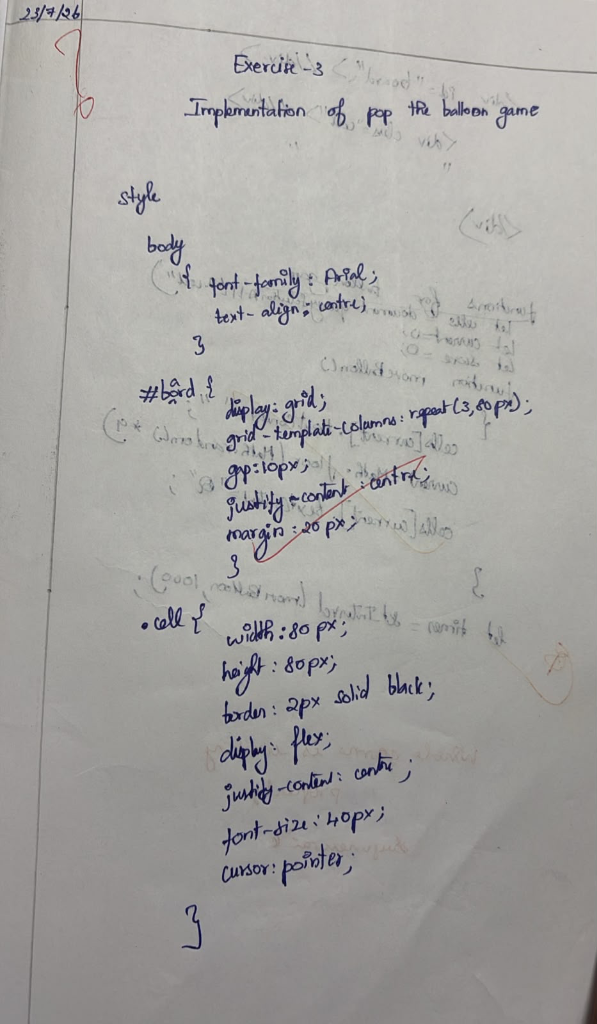
\includegraphics[width=0.74\textwidth,height=0.78\textheight,keepaspectratio]{observation_images/observation_page1.png}
    \caption{Lab Observation Note --- Page 1 (Layout Structure, CSS Grid, and Cell Styling)}
    \label{fig:obs1}
\end{figure}

\newpage

\begin{figure}[H]
    \centering
    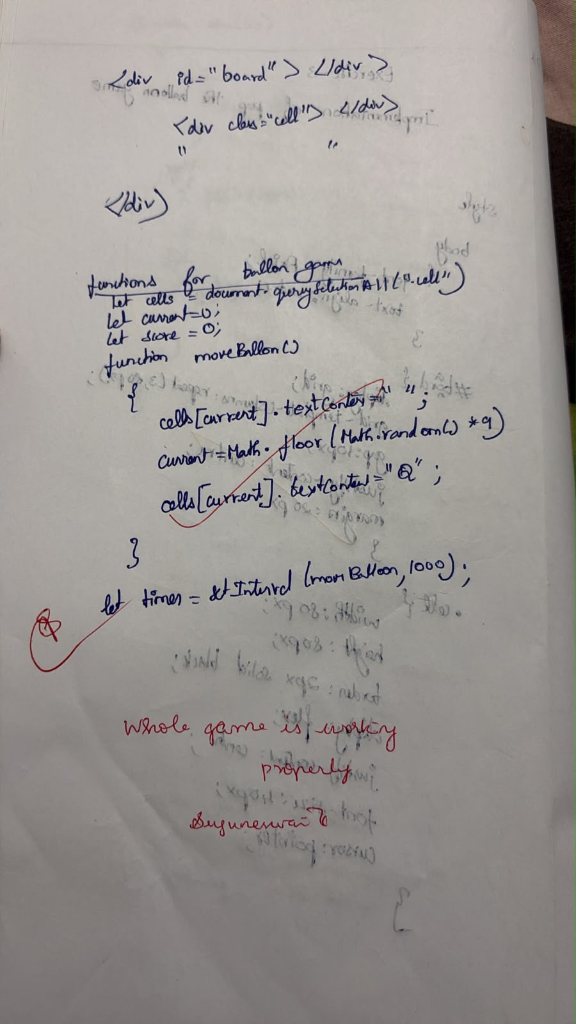
\includegraphics[width=0.74\textwidth,height=0.78\textheight,keepaspectratio]{observation_images/observation_page2.png}
    \caption{Lab Observation Note --- Page 2 (DOM Event Handlers and Verification Sign-off)}
    \label{fig:obs2}
\end{figure}

\newpage

% =========================================================================
% SECTION 3: SOURCE CODE
% =========================================================================
\section{Source Code}

\subsection{1. HTML Structure (\texttt{index.html})}
\lstinputlisting[language=HTML5,caption={Bingo Game Structure (\texttt{index.html})}]{index.html}

\vspace{1.2em}

\subsection{2. Global Stylesheet (\texttt{style.css})}
\lstinputlisting[language=CSS3,caption={Game Stylesheet (\texttt{style.css})}]{style.css}

\newpage

\subsection{3. JavaScript Logic (\texttt{script.js})}
\lstinputlisting[language=JavaScript,caption={Bingo Game Core Mechanics (\texttt{script.js})}]{script.js}

\newpage

% =========================================================================
% SECTION 4: OUTPUT SNAPSHOTS
% =========================================================================
\section{Output Snapshots}

\subsection{1. Initial Game State (Cards Generated)}
\noindent
Upon clicking the \textbf{``Start''} button, randomized $5 \times 5$ grids containing unique values from 1 to 25 are generated for both Player 1 and Player 2, and Player 1 is assigned the active turn.

\begin{figure}[H]
    \centering
    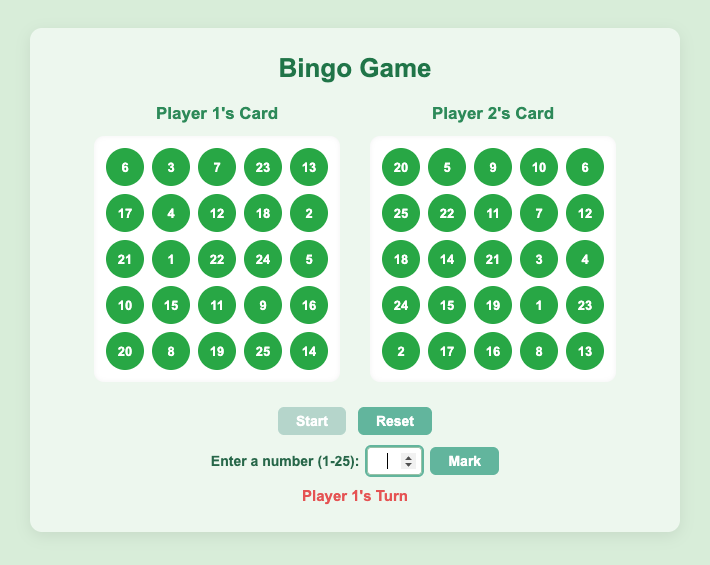
\includegraphics[width=0.88\textwidth]{output_screenshots/initial_game.png}
    \caption{Output Snapshot: Initial State with Randomized Dual Cards (\texttt{index.html})}
    \label{fig:out_initial}
\end{figure}

\vspace{1.0em}

\subsection{2. Game in Progress (Turns and Numbers Marked)}
\noindent
As players take turns entering numbers, the specified values are marked simultaneously on both cards with distinct red circular indicators and the ``X'' symbol.

\begin{figure}[H]
    \centering
    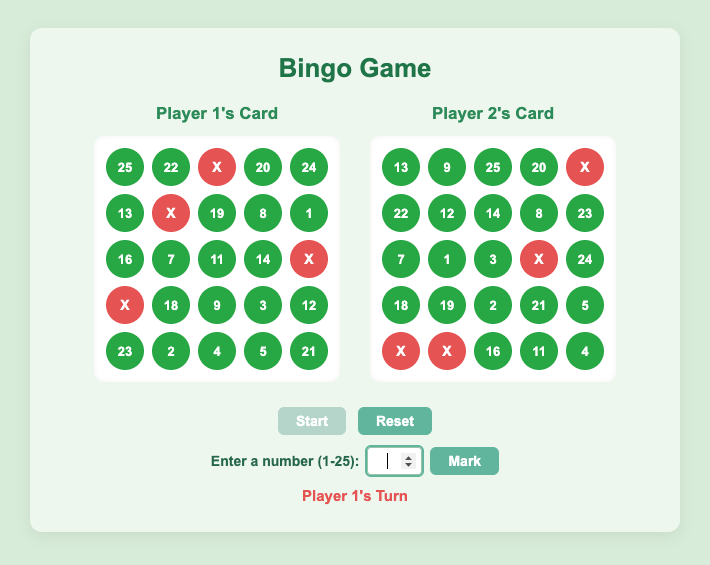
\includegraphics[width=0.88\textwidth]{output_screenshots/in_progress.png}
    \caption{Output Snapshot: Numbers Marked Across Dual Player Cards During Gameplay}
    \label{fig:out_progress}
\end{figure}

\newpage

\subsection{3. Winning State (Bingo Condition Achieved)}
\noindent
When a player completes a full row, column, or diagonal, the winning condition triggers, announcing the winner and disabling the input controls.

\begin{figure}[H]
    \centering
    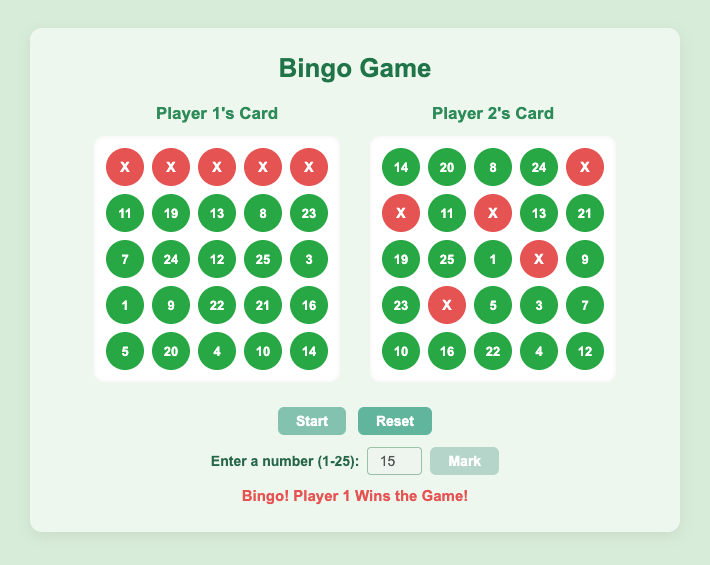
\includegraphics[width=0.88\textwidth]{output_screenshots/winning_state.png}
    \caption{Output Snapshot: Winning State Announcement (Bingo Completed)}
    \label{fig:out_winning}
\end{figure}

\vspace{1.5em}

% =========================================================================
% SECTION 5: LEARNING OUTCOMES & RESULT
% =========================================================================
\section{Learning Outcomes}

Upon successful design, implementation, and verification of this laboratory exercise, the following core learning outcomes were attained:

\begin{enumerate}[leftmargin=*,itemsep=5pt]
    \item \textbf{DOM Manipulation and Dynamic Rendering:} 
    Learned how to dynamically construct and update HTML elements using JavaScript (\texttt{document.createElement}, \texttt{innerHTML}, and \texttt{appendChild}) to render $5 \times 5$ grids from array data structures.
    
    \item \textbf{Array Shuffling and Matrix Representation:} 
    Implemented random array permutation algorithms (Fisher-Yates) to generate unique sets of numbers between 1 and 25, structured into 2D matrices for coordinate-based lookups.
    
    \item \textbf{Event Handling and Input Validation:} 
    Mastered user event capturing using click handlers and keyboard enter listeners, combined with thorough input validation to reject duplicate entries and numbers outside the allowable range.
    
    \item \textbf{Algorithmic Pattern Matching for Win Detection:} 
    Formulated matrix traversal algorithms in JavaScript to evaluate winning conditions across all horizontal rows, vertical columns, and primary/secondary diagonals.
    
    \item \textbf{Turn-Based State Management and Responsive CSS:} 
    Acquired proficiency in synchronizing game states across dual players and styling interactive components using CSS Grid and Flexbox with visual feedback.
\end{enumerate}

\vspace{1.5em}
\section*{Result}
Thus, a fully functional, two-player interactive \textbf{Bingo Game} web application was successfully designed and developed using HTML5, CSS3, and JavaScript in accordance with the laboratory requirements, and the outputs were verified.

\end{document}
